% Template for a Computer Science Tripos Part II project dissertation
\documentclass[12pt,a4paper,twoside,openright]{report}
\usepackage[pdfborder={0 0 0}]{hyperref}    % turns references into hyperlinks
\usepackage[margin=25mm]{geometry}  % adjusts page layout
\usepackage{graphicx}  % allows inclusion of PDF, PNG and JPG images
\usepackage{verbatim}
\usepackage{docmute}   % only needed to allow inclusion of proposal.tex
\usepackage{syntax}
\usepackage{color}
\usepackage{listings}
\usepackage{bussproofs}
\usepackage{tikz}
\usepackage[shellescape,latex]{gmp}
\usepackage{mathtools}
\usepackage{framed}
\usepackage{epstopdf}
\usepackage{mdframed}
\usepackage{changepage}
\usepackage{url}
\usepackage{pdfpages}

\usempxclass{article}
\usetikzlibrary{matrix}
\usempxclass{article}

 % use text width & text height instead of minimum size, as that causes
% alignment issues, and since blocks require uniform sizes
\tikzstyle{tblock} = [matrix of nodes,ampersand replacement=\&,nodes={
    outer sep=0pt,text width=3em,inner ysep=1em,text centered
}]

% \tblock {input} {output} {machine}
\newcommand{\tblocktext}[3]{
    {#1} \& $\to$   \& {#2} \\
    {}     \&  {#3}   \&      \\
}

% \tblock {input} {output} {machine}
\newcommand{\tblocktextnm}[4]{
    {#1} \& {#4}   \& {#2} \\
    {}     \&  {#3}   \&      \\
}

\newcommand{\tblockoutline}[1]{
    \draw (#1-1-1.south west) |- (#1-1-3.north east) |- (#1-1-3.south west) |- (#1-2-2.south west) |- (#1-1-1.south west);
}

\tikzstyle{wblock} = [matrix of nodes,ampersand replacement=\&,nodes={
    outer sep=0pt,text width=3em,inner ysep=1em,text centered
}]

\newcommand{\wblocktext}[1]{
    {#1} \\
    {}\\
}

\newcommand{\wblockoutline}[1]{
    \draw (#1-1-1.south west) |- (#1-1-1.north east) -- (#1-1-1.south east) -- (#1-2-1.south) -- (#1-1-1.south west);
}

\tikzstyle{vblock} = [matrix of nodes,ampersand replacement=\&,nodes={
    outer sep=0pt,text width=3em,inner ysep=1em,text centered
}]

% \vblock {supports} {depends}
\newcommand{\vblocktext}[2]{
    	{#1} 	\\
      			\\
	{#2}	\\
}

\newcommand{\vblockoutline}[1]{
	\draw (#1-1-1.north west) |- (#1-3-1.south east) |-  (#1-1-1.north west);
}

\tikzstyle{pblock} = [matrix of nodes,ampersand replacement=\&,nodes={
    outer sep=0pt,text width=3em,inner ysep=1em,text centered
}]

% \vblock {name} {language}
\newcommand{\pblocktext}[2]{
    	{#1} 	\\
	{#2}	\\
}

\newcommand{\pblockoutline}[1]{
	\draw (#1-1-1.north west) arc [radius=0.55, start angle=90, end angle = 270];
	\draw (#1-1-1.south east) arc [radius=0.55, start angle=270, end angle = 450];
	\draw (#1-1-1.north west) -- (#1-1-1.north east);
	\draw (#1-1-1.south east) |- (#1-2-1.south west)  |-  (#1-2-1.north west);
}

\newcommand{\wsupt}[2]{
	\node(mac#2) at (#2-2-2.south west) [wblock, anchor = mac#2-1-1.north west] {\wblocktext{#1}};
	\wblockoutline{mac#2};
}

\raggedbottom                           % try to avoid widows and orphans
\sloppy
\clubpenalty1000%
\widowpenalty1000%

\renewcommand{\baselinestretch}{1.1}    % adjust line spacing to make
                                        % more readable

\begin{document}
\EnableBpAbbreviations
\makeatletter \renewcommand{\@cite}[1]{\textsuperscript{\,[#1]}} \makeatother

\bibliographystyle{plain}

\lstset{language=Prolog}
\lstset{showstringspaces=false}
\lstset{basicstyle=\tt}
 
%%%%%%%%%%%%%%%%%%%%%%%%%%%%%%%%%%%%%%%%%%%%%%%%%%%%%%%%%%%%%%%%%%%%%%%%
% Title


\pagestyle{empty}

\rightline{\LARGE \textbf{Lawrence Esswood}}

\vspace*{60mm}
\begin{center}
\Huge
\textbf{Object Oriented Prolog Compiler} \\[5mm]
Computer Science Tripos -- Part II \\[5mm]
Churchill College \\[5mm]
\today  % today's date
\end{center}

%%%%%%%%%%%%%%%%%%%%%%%%%%%%%%%%%%%%%%%%%%%%%%%%%%%%%%%%%%%%%%%%%%%%%%%%%%%%%%
% Proforma, table of contents and list of figures
%/


\pagestyle{plain}

\chapter*{Proforma}

{\large
\begin{tabular}{ll}
Name:               & \bf Lawrence Esswood                       \\
College:            & \bf Churchill College                     \\
Project Title:      & \bf Object Oriented Prolog Compiler \\
Examination:        & \bf Computer Science Tripos -- Part II, July 2015  \\
Word Count:         & \bf 10615 \\
Project Originator: & Lawrence Esswood                    \\
Supervisor:         & Dr Alan Mycroft                    \\ 
\end{tabular}
}
\stepcounter{footnote}


\section*{Original Aims of the Project}

The aims of the project were to produce a bootstrapping compiler that takes an Object-Oriented Dialect of Prolog and produces Prolog as an output. The Compiler should, at the least, be able to handle the definition of classes, fields and predicates within classes. The language should provide polymorphism by way of late binding predicates. As an optional extension multiple inheritance, inner classes, and access modifiers could be added to the language.

\section*{Work Completed}

A variant of Prolog, OOPL, was devised. A compiler, interpreter and runtime for OOPL were implemented, all in the OOPL language. The compiler supports the definition of classes with fields, predicates and an optional parent class, but not multiple inheritance. Classes inherit fields and predicates from parent classes, fields can be pattern-matched like Prolog variables, and predicates with the same name can be defined in multiple classes without conflict.

\section*{Special Difficulties}

None.
 
\newpage
\section*{Declaration}

I, Lawrence Esswood of Churchill College, being a candidate for Part II of the Computer
Science Tripos, hereby declare that this dissertation and the work described in it are my own work,
unaided except as may be specified below, and that the dissertation
does not contain material that has already been used to any substantial
extent for a comparable purpose.

\bigskip
\leftline{Signed }

\medskip
\leftline{Date }

\tableofcontents

\listoffigures

\newpage
\section*{Acknowledgements}

Many thanks to Alan Mycroft, for his advice and guidance during the course of this project, John Fawcett for teaching me the past few years, and Tom Rees for repeatedly reading this document.

%%%%%%%%%%%%%%%%%%%%%%%%%%%%%%%%%%%%%%%%%%%%%%%%%%%%%%%%%%%%%%%%%%%%%%%
% now for the chapters

\pagestyle{headings}

\chapter{Introduction}

\section{Background and Motivation}

The aim of modern programing languages is to provide programmers with powerful abstractions that allow complicated algorithms and structures to be implemented with maximum efficiency and minimal errors. Compilers provide the mechanism for translating between languages and are a necessity to bridge the gap between the high-level languages used by programmers and the languages our machines are designed to run. Furthermore, compilers can perform transformations that, while retaining semantic behaviour, produce smaller, more efficient, or otherwise more desirable output. As such compilers continue to be a large, active area of research.

\bigskip

Prolog is a declarative language based on first-order logic. It has proven a very powerful language for certain applications such as artificial intelligence\cite{AIBOOK} and natural language programming\cite{NLPBOOK}. However it is missing many features that are necessary for programming in the large. Modules in Prolog go some way to providing these features, but fall short in some aspects. For example, there is no way of providing information-hiding, polymorphism or inheritance using modules.

\bigskip

Object Oriented Programing (OOP) is a paradigm that can be found in many, mostly procedural, languages. Objects combine state and method and are a good way of separating interface and implementation. They can provide an effective way of building larger, more robust systems. Because of this objects could prove a useful addition to the Prolog language. A practical way of exploring the use of objects in Prolog is to construct a compiler for a modified version of language.

\section{Work Undertaken}

A new language Object Oriented Prolog (OOPL) was designed with a view to introducing class-based object-oriented programing to Prolog while keeping as much of the semantics the same as possible. A bootstrapping compiler was written in its own language, targeting Prolog as a back end. The bootstrapping was facilitated using a basic version of the compiler written in Prolog, see more in the implementation section.

\subsection {OOPL Example}

\begin{lstlisting}
% A class representing a 2D vector. %
class vector. 
	X. Y. % Fields.
	vector(X, Y). % Constructor. %
	
	 % A sum predicate. %
	sum(V2, V3) :- 
		X3 is X + V2::'X',
		Y3 is Y + V2::'Y',
		new(vector, V3, X3, Y3).
		
	% A magnitude predicate. %
	magnitude(M) :- M is sqrt((X * X) + (Y * Y)). 
endclass.
\end{lstlisting}

\section{Related Work}

Extending existing languages with Object-Oriented features is nothing new, in fact one of the most historically popular languages ,C++, was first envisioned as a `C with Classes'\cite{CPP}. There have also been several previous successful attempts to extend the Prolog language with object oriented-concepts:

\bigskip

One of these attempts, SCOOP\cite{SCOOP},  takes the same approach of class-based inheritance as OOPL\@. SCOOP takes its inspiration for OOP from Simula67 and uses very conventional OOP syntax for global behaviour, while using unification and backtracking for local behaviour. Rather than explicitly providing fields, assert and retract predicates are used to provide state.

\bigskip

Logtalk\cite{LOGTALK} provides a more fleshed out implementation, providing both class-based and prototype-based systems, and multiple inheritance. It also uses assert and retract predicates to provide mutable state to objects. 

\bigskip

My implementation takes a different approach to providing state by way of explicit fields, which are similar to variables in that they can be used for pattern-matching and unification is used for instantiation. This maintains the behaviour of Prolog while still providing a syntactic method for declaring state other than predicates. Also the mechanism for inheritance differs from most OOP languages in that overriding extends behaviour, this is similar to how Prolog allows multiple clauses with the same name, more detail is given in preparation chapter. The motivation for taking this direction was to merge OOP concepts with Prolog, rather than create an extension that operates in a different manner.

\chapter{Preparation}

This section covers the planning sections of the project and the development methods used. It also provides some background on the topics relevant to the project such as the Prolog language and bootstrapping.

\section{Starting Point}

While studying the tripos course I have been introduced to both object-oriented programing and basic Prolog programing. Furthermore I have taken two compilers courses and undertaken some summer reading on compilers, namely `Aho, Sethi, Ullman'\cite{DRAGON}.

\section {Language Design}
\label{sec:lang}
Although the focus of the project was to create a compiler, the choice was made to design a novel extension to Prolog rather than copy existing implementations such as SCOOP, SICStus and Logtalk. This choice was made as it was interesting to explore different options and design decisions and compare results. The choice was made to provide class-based as opposed to prototype-based objects as it leave the way open for better static analysis. My OOPL language is an extension to Prolog, as such every Prolog program is still valid in OOPL. Below a simple introduction to the syntax and semantics of Prolog is given, and the extensions that have been added to create OOPL.

\subsection {Syntax}

The abstract syntax of a language is most readily described as a context free-grammar. A dot character followed by any whitespace character is used to end a clause, it is just written as a `.' below. Provided below is a context free-grammar for Prolog. It should be noted that Prolog has a very simple syntax.

\begin{grammar}

<program> ::= <def>*
		
<def> ::= <clause>
		
<clause> ::= <head> `:-' <body> `.'
		
<head> 	::= <pred> `(' <term>* `)'
		
<body> ::= <head>*

<query> ::= `?-' <body>

\end{grammar}		

A Prolog program consists of number of clauses. We normally split these into two categories, a clause with an empty body is a \emph{fact}, otherwise we call it \emph{rule}. We normally omit writing the `:-' for facts. A query is used to begin execution of a Prolog program, execution is covered in the semantics section.

\begin{grammar}	
				
<term> ::= <variable>
\alt <functor> `(' <term>* `)'

\end{grammar}

Prolog has 3 types of term, $\langle$term$\rangle$ in the abstract syntax. Atoms are a particular form of ground term, they are alphanumeric and must either start with a lower case letter or be quoted. A Compound is composed of an atom called a \emph{functor} and a number of arguments which are again terms. The number of arguments is known as the compounds \emph{arity}. Atoms are treated as compounds of arity zero, and hence are not mentioned separately. Variables, $\langle$variable$\rangle$, are placeholders for arbitrary terms, they are also alphanumeric and must start with either a capital letter or underscore.

\bigskip

To introduce the additional syntax of OOPL we add the following:

\begin{grammar}
<def> ::= <field>
\alt <class>
\end{grammar}

We add two more definitions for the programmer to use, a field or a class. These can appear anywhere a clause would, although the language will reject fields outside of a class.

\begin{grammar}
<field> ::= <variable> `.'
\end{grammar}

Fields are named the same way as variables, they must start with a capital letter or underscore.

\begin{grammar}
<class> ::= <header> `.' <def>* `endclass' `.'

<header> ::= `class' <atom>
\alt `class' <atom> `extends' <atom>*
\end{grammar}

Classes are named in the same way as atoms and can optionally extend some number of classes. The body of the class can consist of any number of definitions including fields, predicates and other classes. 

\begin{grammar}
<functor> ::= `new'

<infix> ::= `::'
\end{grammar}

We introduce a functor called \emph{new} and a macro \emph{::} that is written infix. The first is used to construct objects, the second to access their members. The detailed semantics of these two operators are given below.

\subsection {Semantics}

Provided here is an informal introduction to the semantics of Prolog as well as the new features added and how they change the semantics.

\subsubsection {Predicate Description Notation}

Throughout this document predicates and their arguments will be given with a standard notation. Firstly the notation `P/n' means a predicate that has a name `P' and `n' arguments. If the arguments are named, then each will preceded by a symbol with the following meaning attached (This is taken from the SWI-Prolog documentation\cite{SWIDOC}, Chapter 4.1):

\begin{itemize}
	\item + Argument must be fully instantiated to a term that satisfies the required argument type. Think of the argument as input.
	\item - Argument must be unbound. Think of the argument as output. 
	\item ? Argument must be bound to a partial term of the indicated type. Note that a variable is a partial term for any type. Think of the argument as either input or output or both input and output.
\end{itemize}

Note that inputs need not be ground terms, and it is perfectly acceptable to provide a bound term as an output to check for a particular result.

\subsubsection {Prolog}

A Prolog program, \emph{P}, is a number of Horn clauses ( $\langle$clause$\rangle$ in the syntax), a subset of first-order predicate logic. The clauses define a set of axioms within a closed universe. A clause of the form $a$ :- $\vec{b}$, where $\vec{b}$ = $b_1, b_2, ..., b_n$, should be seen as the logical implication $a \leftarrow b_1 \land b_2 \land ... \land b_n$. 

\bigskip

Unification of terms is a very important concept in Prolog as execution is performed by attempting unification of terms and backtracking. The rules for unification are as follows:

\begin{itemize}
	\item A Variable unifies with any other term\footnote{If the occurs check is turned on, unification will fail if the variable appears as a subterm in the term you attempt you unify with.}.
 	\item A Compound unifies with another Compound if and only if they have the same functor and arity, and their arguments can be pairwise recursively unified.
\end{itemize}

We will define a function, MGU(X, Y), which returns the most general unifier of terms X and Y, or fails if they do not unify.

\bigskip

Users start the execution of a program by submitting a single goal, known as a query, which is of the form ?-q $ = (q_1 \land ... \land q_n)$. Prolog attempts to find some way to satisfy the query, returning the substitutions it makes as a result, otherwise it fails. The strategy Prolog employs is called SLD resolution and works on the premise of attempting to refute the negation of the query. A depth-first left-right search over the axioms of the program is the strategy employed by most Prolog interpreters for efficiency reasons. This is only weakly complete, that is if it terminates then it is complete, but non-termination may occur even when a refutation exists. From this we can obtain the following operational semantics based on those given by Mycroft and Jones\cite{MYCROFT}.

\bigskip

We use a stack not to record function calls but to keep track of state so that we can backtrack if necessary. Each element on the stack is formed of a 3-tuple. The first is a conjunction of as-yet-unsatisfied goals, the second is the composition of all the MGU substitution functions so far, and the third is the remaining clauses we can try to apply. We start with a stack with a single element containing the list of goals that is the query, \emph{g}, the identify substitution, \emph{ID}, and the entire program, \emph{P}, as the set of available clauses to apply. The Start State:

\bigskip

StartState = (q, ID, P) : [\,]

\bigskip

I have used colon for cons, to avoid confusion with the :: operator defined later. The `@' symbol is used below to refer to list append, and `[\,]' is the empty list. The transition relation, \emph{$\to$} between states is described below:

\begin{prooftree}
\AXC{}
\RightLabel{where $\theta = MGU(a, a')$}
\LeftLabel{(apply clause)}
\UIC{($a : \vec{b}, \phi, (a' \leftarrow \vec{b}'): C) : stack \to$ }
	\noLine
\UIC{($\theta(\vec{b}') @ \theta(\vec{b}), \theta\circ\phi, P) :  (a : \vec{b},  \phi, C) : stack$}
\end{prooftree}
This is the case where the current clause\footnotemark\,under consideration unifies with the left-most goal. We pop off the top element on the stack and replace it with two more: a backtracking point in case we fail later on later, and an element where the clause has been successfully applied.
\footnotetext{Technically $a\leftarrow\vec{b}$ is renamed apart to use fresh variables.}
\begin{prooftree}
\AXC{}
\RightLabel{where $MGU(a, a')$ fails}
\LeftLabel{(clause does not unify)}
\UIC{($a : \vec{b}, \phi, (a' \leftarrow \vec{b}') : C) : stack \to$}
\noLine
\UIC{$(a : \vec{b}, \phi, C) : stack$}
\end{prooftree}
If we cannot apply the current clause we remove it from the list and continue on.
\begin{prooftree}
\AXC{}
\LeftLabel{(backtrack)}
\UIC{$(g, \phi, [\,]) : stack \to stack$}
\end{prooftree}
If there are no more clauses left to try we backtrack by popping an element off the stack.
\begin{prooftree}
\AXC{}
\LeftLabel{(fail)}
\UIC{[\,] $\xrightarrow{fail}$ [\,]}
\end{prooftree}
If we reach the bottom of the stack then there are no more ways to satisfy the query, and we fail and execution stops.
\begin{prooftree}
\AXC{}
\LeftLabel{(output)}
\UIC{([\,],  $\phi$, C) : stack $\xrightarrow{true, \phi}$ stack}
\end{prooftree}	
If ever reach a state no goals remaining, we have found a solution. We output the final substitutions that apply to the original variables in the query as the result. At this point we can also forcibly backtrack, finding all the remaining (potentially infinite in number) solutions.

\bigskip

There is also a special operator `!' in Prolog called a cut. When Prolog encounters a cut within the body of a clause, it will limit backtracking so that none of the goals within the body, nor the head of the clause, can be retried. A more formal description can be found in \cite{MYCROFT}.

\bigskip

The above semantics were extended to add classes. The details of each new feature is given below.

\subsubsection {Objects}

Objects are a new form of Prolog term, distinct from atoms, compounds, and variables. They are always instances of a particular class created using the \emph{new} syntax (see later). To update the semantics, we change the MGU function above such that we also include the following rules for unification:

\begin{itemize}
	\item A Variable and an Object can always be unified.
	\item An Object and an Object can be unified if and only if they are instances of the same class and each of their fields can be recursively unified\footnote{In most OOP languages (e.g. Java) objects have identity. This is not true in OOPL due to the way we unify objects.}.
	\item An Object cannot be unified with a compound.
\end{itemize}

\subsubsection {Classes}

A class gives a description of an object and lists the fields an object will have as well as the concrete implementation of its member predicates. Within the class any predicate with the same name as the class is given special meaning as a \emph{Constructor}. Constructors cannot be used as goals directly, doing so will produce a compile-time error. Instead constructors are implicit goals when the \emph{new} predicate is applied, see below.

\bigskip

Every predicate within a class can use an implicit variable called \emph{This}. \emph{This} will always be bound at run time to the instance of a class from which the predicate was accessed. For example take the following snippet.

\begin{lstlisting}
class a.
	foo :- write(This). % A simple member predicate
endclass.

bar :- new(a, Ob), % Constructs a new a, binds it to Ob
	call(Ob::'foo'). % Accesses and invokes foo
\end{lstlisting}

Invoking the \emph{bar} predicate calls\footnote{The inbuilt \emph{call} predicate in Prolog takes a compound and attempts to satisfy it as a goal} \emph{foo}. Within the call to \emph{foo} the \emph{This} variable is unified with \emph{Ob}.

\bigskip

Notice in the above example an atom \emph{a} was used to refer to the class when using `new'. At any scope where the class's definition is visible using an atom with the same name as the class will instead give a value representing the class. Classes are first-class citizens in OOPL and are represented by an object at runtime of class classType\footnote{In a similar way to Java in which we can use reflection to get an object of type `Class'.}. It would have therefore been legal to have written ``X = a, new(X, Ob)'' and the same result should be expected.

\subsubsection {Inheritance}

Inheritance allows a child class to inherit all the fields and predicates of a parent class. In most object-oriented languages redefining a virtual method (the equivalent of a predicate in OOPL) in a child that is also present in the parent class will \emph{override} behavior. Selecting which method to use at runtime is known as dynamic dispatch. In OOPL all predicates within classes are by default virtual, however with one crucial difference in that if a predicate fails in the child, the parent's version is tried. This keeps the semantics more in line with how Prolog would normally handle multiple predicates of the same name, \emph{overriding adds to behaviour}. In the case of multiple inheritance we again try all implementations of the predicate, trying them the order the parents were listed after the `extends' keyword, in a depth first fashion. If the programmer wishes to override its parents in the classical sense, a cut can be used.

\subsubsection {Scope}

The \emph{Scope} of some named thing refers to the places in a program from which it can be referred to. Scopes are nested in a tree-like structure. The top-level scope contains all the predicates not within a class. Each class creates a new scope, and is enclosed by the scope in which it was defined (either the top scope, or another class's scope in the case of inner classes).

\bigskip

Defining a predicate with the same name as in another scope shadows the outer predicate. If a class extends another all the fields and predicates it inherits are considered to be in the current scope. When we look up a name to see what it resolves to we first check the current scope, then any enclosing scope and so on. We take the first match as the resolved name. For example consider the following code fragment:

\begin{lstlisting}
foo. % Top level predicate

class a.
	foo. % Member predicate of the same name
endclass.

class b.
	foo. % Member predicate of the same name
	class c extends a.
	endclass.
	class d.
	endclass.
endclass.

class e.
endclass.

\end{lstlisting}


\noindent Using the atom foo in different places will have the following meaning

\begin{center}
\begin{tabular}{c|c}
Place Used & `foo' refers to \\
\hline
top & top \\
a & a \\
b & b \\
c & a \\
d & b \\
e & top \\
\end{tabular}
\end{center}

Every scope that defines the \emph{foo} predicate simply uses its own verion (i.e. top, a and b). Class c uses the version from a as it is a child class of a. Classes d and e use the version defined in their enclosing scope. In this way we do not have to worry about reusing names of predicates, a class can contain a predicate that is a duplicate and have it completely hidden outside of the class's scope.

\subsubsection {New}

The \emph{new/n} variable-length predicate is used to create a new instance of object. It is a relation between a class, an instance, and a number of terms to provided to the constructor. Classes are represented at runtime as objects of class `classType'. If Cl is some runtime representation of a class, with a constructor called `con' then the goal ``new(Cl, Ob, $T_1$, ..., $T_n$)'' succeeds if and only if Ob can be unified with a new, empty, instance of Cl and the goal ``con($T_1$, ..., $T_n$)'' within Ob succeeds. new/n will attempt unification via backtracking for every constructor of the class with the correct arity (any unification/construction that occurs will be undone upon backtracking), this is in contrast to inheritance where we would also try the parents definitions.

\bigskip

Let \emph{Instance} be a mathematical function that takes a class as an argument and returns an object that is an instance of that class that is renamed apart\footnote{A clause/object is \emph{renamed apart} if its variables, including fields, do not occur elsewhere}. In terms of the operational semantics of Prolog given above, we now have an additional case where the left-most goal is the \emph{new} predicate. This uses the \emph{access/3} predicate introduced later.

\begin{prooftree}
\AXC{}
\RightLabel{where $\theta$ = MGU(Ob, Instance(Cl))}
\LeftLabel{(new)}
\UIC{(new(Cl, Ob, $T_1, ..., T_n$ )) : b, $\phi$, C) : stack $\to$ }
	\noLine
\UIC{($\theta$(access(Cl, `Constructor', con)) : $\theta$(con(Ob, $T_1, ..., T_n$ )) : $\theta$b, $\theta\circ\phi$, P) : stack}
\end{prooftree}

Although not explicit here, it is the access/3 predicate that will provide backtracking via the normal Prolog backtracking rule. The Semantics of the access/3 predicate are discussed below. 

\subsubsection {Fields}

In OOPL fields defined within a class act like variables. They are visible to any predicate within the class, unless they are shadowed by another variable. If any predicate unifies the variable the substitution is visible from any other predicate in scope, and if backtracking occurs the unification is undone in the same way.

\bigskip

In this way objects in OOPL are mutable in that we can unify variables with other Terms, but only insofar as normal Prolog variables can be substituted for other terms. 

\subsubsection{Accessing Fields}

Sometimes the programmer may want to inspect the internal state of an object. In line with Prolog defining a universe in terms of relations, accessing a member of a class is a relation between the instance of the class, the name of the fields, and its value. Let this relation be a predicate called access/3 such that the goal ``access(Object,Field,Value)'' is satisfiable only when `Object' is an object with a field called `Field' with value `Value'.

\bigskip

We can provide unbound variables to both Field and Value (although currently Object must be bound) and OOPL will attempt to unify them with any matching field-value pair, successively trying all combinations until it fails. 

\bigskip
Although this is the underlying mechanism for accessing a member of a class, it was considered too verbose. e.g. consider accessing a deeply nested value like so: 
\begin{lstlisting}
access(V1,F1,V2), access(V2, F2, V3), access(V3, F3, Res).
\end{lstlisting}
To avoid this OOPL provides the `::' infix operator. X::Y is a syntactic term which is automatically evaluated such that access(X, Y, X::Y) holds true. The example given above can now be written as:
\begin{lstlisting}
Res = V1::F1::F2::F3.
\end{lstlisting}

\bigskip

This makes the semantics of goals that contain a term with the :: operator different from most operators in Prolog. A parallel might be drawn with using arithmetic operators. The term 1+1 is not the same as the term 2, and if the user wishes to evaluate a term the \emph{is} operator must be used. With the :: operator however terms are automatically evaluated, even if deeply nested within compound structures. This was motivated by a desire to reduce the quantity of required syntax to use the OOP features provided by OOPL. Using the [X/Y] notation to denote the substitution function of `X for Y', and A $\in$ B to mean that the syntactic term A appears somewhere within compound term B we add one further rule:

\begin{prooftree}
\AXC{}
\RightLabel{where X::Y $\in$ a}
\LeftLabel{(access)}
\UIC{(a : b, $\phi$, C) : stack $\to$ }
	\noLine
\UIC{(access(X, Y, Z) : [Z/X::Y]a : [Z/X::Y]b, [Z/X::Y]$\circ\phi$, P) : stack}
\end{prooftree}

\subsubsection{Accessing Member Predicates}

OOPL does not distinguish between accessing fields and accessing member predicates, and the exact same `::' syntax is used for both. The name by which we access a predicate is the atomic name of the predicate. The result of accessing a member predicate from an object is a term that can be used with the Prolog call predicate. As previously mentioned, when invoked the `This' variable is dynamically bound to the instance from which the the predicate was accessed. Therefore the result of accessing a predicate from an object can be viewed as returning a closure of the predicate with the object.

\section{Tombstone Diagrams}
	Tombstone diagrams offer an intuitive way of describing compilers, especially when considering bootstrapping. They were first described by McKeenman in `A Compiler Generator'\cite{TOMB}. As they are used throughout this document a quick description is given here.

\bigskip

Tombstone diagrams are made up from a number of building blocks. Examples of each tombstone block:

\bigskip

\begin{tikzpicture}
    %\node(right) at (mid-1-3.north west) [tblock,anchor=right-1-1.south west] {\tblocktext{C}{M}{M}};

	\node(compiler) [tblock] {\tblocktext{A}{B}{C}};
	\tblockoutline{compiler};
    	
    	\node(translate) at (4,0) [vblock] {\vblocktext{D}{E}};
    	\vblockoutline{translate};
    	
    	\node(prog) at (8,0) [pblock] {\pblocktext{P}{L}};
    	\pblockoutline{prog};
    	
    	\node(bottom) at (12,0) [wblock] {\wblocktext{M}};
    	\wblockoutline{bottom};
    	
\end{tikzpicture}

From left to right:

 \begin{itemize}
 	\item A compiler that translates from language A to language B, written in language C.
 	\item An interpreter that runs language D, implemented in language E.
 	\item A program P, typically not a compiler, written in language L.
 	\item A machine that can natively run language M.
\end{itemize}

A diagram is built by connecting pieces together with matching languages. To represent running a program, we place one block on top of the other. To represent translating a program, we place the source program to the left of the compiler block, and the target to the right. A correct diagram should have all of its foundations be machines, and have all connections match languages.

 \bigskip
 
An example using all the blocks that shows how we might compile a Java program to ByteCode and then interpret this, all on an x86 machine:

\begin{center}
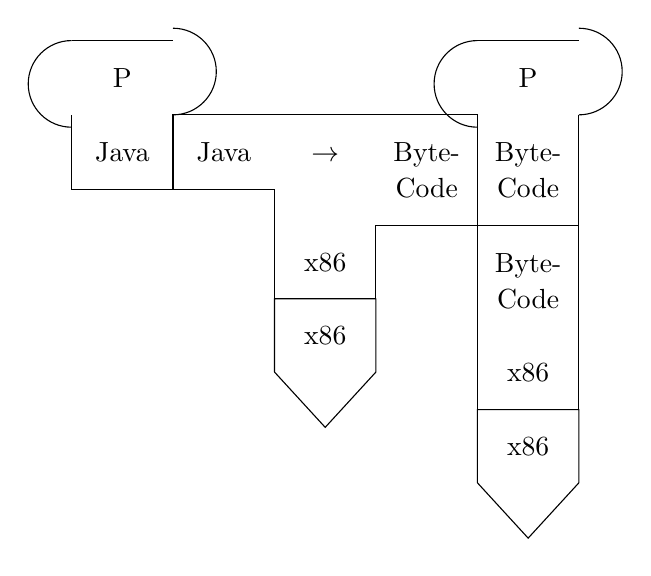
\begin{tikzpicture}
	\node(compiler) [tblock] {\tblocktext{Java}{Byte-Code}{x86}};
	\tblockoutline{compiler};
	
	\node(prog1) at (compiler-1-1.north west) [pblock, anchor = prog1-2-1.north east] {\pblocktext{P}{Java}};
	\pblockoutline{prog1};
	
	\node(prog2) at (compiler-1-3.north east) [pblock, anchor = prog2-2-1.north west] {\pblocktext{P}{Byte-Code}};
	\pblockoutline{prog2};
	
	\wsupt{x86}{compiler};
	
	\node(inter) at (prog2-2-1.south west) [vblock, anchor = inter-1-1.north west] {\vblocktext{Byte-Code}{x86}};
	\vblockoutline{inter};
	
	\node(mac2) at (inter-3-1.south west) [wblock, anchor = mac2-1-1.north west] {\wblocktext{x86}};
	\wblockoutline{mac2};
\end{tikzpicture}
\end{center}

\subsection{Bootstrapping A Compiler}
	
A neat way of producing a compiler is to write it in its own language. For example our compiler for OOPL that targets Prolog looks like this:

\begin{center}
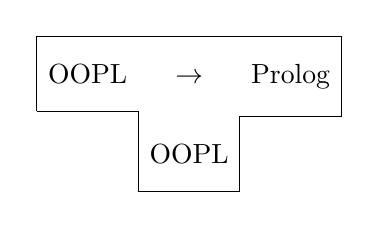
\begin{tikzpicture}
	\node(compiler) [tblock] {\tblocktext{OOPL}{Prolog}{OOPL}};
	\tblockoutline{compiler};
\end{tikzpicture}
\end{center}

This is particularly good as we do not have to rely on any other languages and can continuously upgrade and use new features as they appear. This poses the problem however of how to first run the compiler on itself. The answer is to use another compiler to start the process, and then run the result on itself again and again until we reach a fixed point which is independent of the compiler we used to start the process.

 \bigskip
 
For example, using an OOPL to Prolog compiler written in Prolog to bootstrap the above compiler, then running it on itself:

\begin{center}
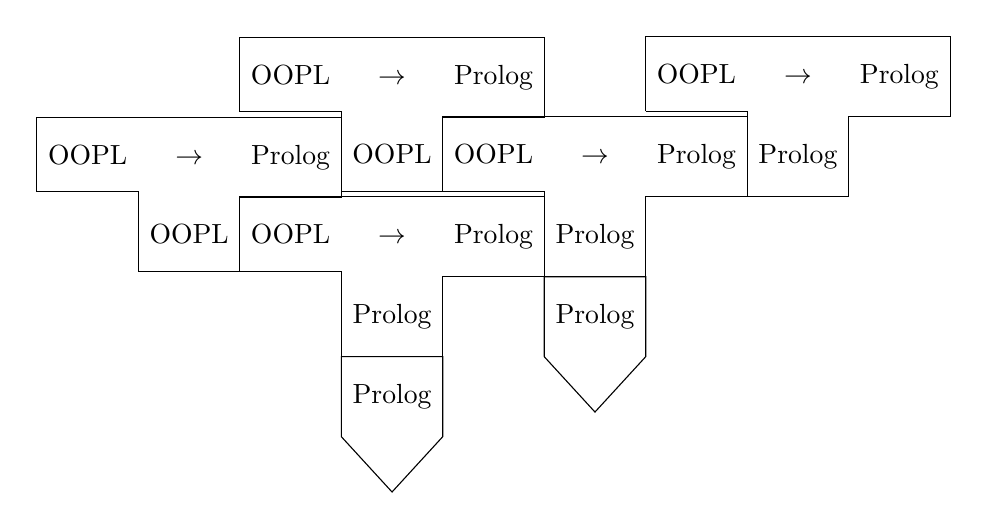
\begin{tikzpicture}
	\node(compiler1) [tblock] {\tblocktext{OOPL}{Prolog}{Prolog}};
	\tblockoutline{compiler1};
	
	\node(compiler2) at (compiler1-1-1.north west) [tblock, anchor = compiler2-2-2.north east] {\tblocktext{OOPL}{Prolog}{OOPL}};
	\tblockoutline{compiler2};
	
	\node(compiler3) at (compiler1-1-3.north east) [tblock, anchor = compiler3-2-2.north west] {\tblocktext{OOPL}{Prolog}{Prolog}};
	\tblockoutline{compiler3};
	
	\node(compiler4) at (compiler3-1-1.north west) [tblock, anchor = compiler4-2-2.north east] {\tblocktext{OOPL}{Prolog}{OOPL}};
	\tblockoutline{compiler4};
	
	\node(compiler5) at (compiler3-1-3.north east) [tblock, anchor = compiler5-2-2.north west] {\tblocktext{OOPL}{Prolog}{Prolog}};
	\tblockoutline{compiler5};
	
	\wsupt{Prolog}{compiler1};
	\wsupt{Prolog}{compiler3};
\end{tikzpicture}
\end{center}

Gives us a compiler that should be the same as if we had somehow been able to run our compiler on itself using a machine natively able to run OOPL. It is however possible to reach a fixed point but a still get an incorrect version of the compiler, whether by a bug in the first compiler or malicious insertion of a compiler back-door that propagated down the chain of compilers. This attack was first reported in an air-force critique\cite{MULTICS} and later popularized by Ken Thompson in his Turing Award acceptance speech\cite{KEN}. Therefore it should be obvious that the correctness of the compiler depends not only on the final source code, but intermediate compilers which are harder to analyse. This factored into the reasoning for testing the compiler with a corpus of small programs.

\section{Requirements Analysis}
\label{sec:req}
In order to keep the project on schedule while maintaining opportunities for adding more features if the project moved faster than planned the MOSCOW method was employed. The following table illustrates planned features and categorizes them as a (M)ust have, (S)hould have, (C)ould have or (W)ould have.

\subsubsection{Must}

\begin{itemize}
	\item Handle the definition of classes and also resolve references to the class within predicates.
	\item Handle the definition of predicates (including constructor predicates) within classes and be able to correctly resolve which predicate to use with scoping rules.
	\item Allow fields within classes and pattern match with them.
	\item Allow optional single inheritance of both fields and predicates in a manner specified in the semantics section.
	\item Support the `::' syntax for member access to return both fields and predicates of a class.
	\item Support the `new' predicate to construct a class and call its constructor.
\end{itemize}


\subsubsection{Should}
\begin{itemize}
	\item Provide compile-time error and warning messages, e.g. trying to inherit from a class that does not exist.
	\item Allow access modifiers such as `Public' and `Private' that restrict access to class members.
	\item Allow static fields and predicates that are shared between instances of a class.
\end{itemize}

\subsubsection{Could}
\begin{itemize}
	\item Allow classes to inherit from multiple parents.
	\item Optimise dynamic binding using a hash table.
\end{itemize}

\subsubsection{Would}
\begin{itemize}
	\item Allow functional style methods in classes.
	\item Perform compiler-time type checking to provide further optimisations.
\end{itemize}

\section{Development Process}

Before any work was undertaken it was important to choose a set of development tools and development methodologies to avoid potential problems further down the road. The software used to develop and maintain the project is given below, as well as the techniques used for development.

\subsection{Choice of software}

A number of suitable software tools were employed to make efficient use of time during development. Sublime Text was used as an editor. A GIT repository was maintained to provide source control and the repository was backed up using GitHub. The build scripts responsible for bootstrapping the compiler were written in Prolog, and the entire project used SWI-Prolog as both an interpreter for the back-end Prolog and as a debugging environment.

\bigskip

The revision control provided by GIT was particularly important for managing the development of the bootstrapping compiler as safe checkpoints were needed at each stage. Without this an accident during development may have lead to a correctly written final compiler but no way of compiling it as one bootstrapping stages in the middle was lost.

\bigskip

It was not necessary to find any libraries to support the project as the Prolog standard includes a large number of very powerful predicates to provide most functionality required, including lexing and parsing.

\subsection{Software techniques}

An Incremental Development methodology was employed during development. This made a large amount of sense due to the nature of bootstrapping. In order to add new features a working version of the compiler was required to be created and tested at each iteration of development. Furthermore some prototyping was applied in that an initial version of the compiler had to be designed in a different language to start the bootstrapping process.

\bigskip

During the testing stages of the project a number of unit tests were created in Prolog to both test new features and to guard against regression. 

\section {Summary}

An outline of Prolog and an extension for it, OOPL, has been given. OOPL adds the ability to define, construct, and manipulate objects in a Prolog setting. Furthermore, the process of bootstrapping a compiler has been outlined. In the next chapter the implementation of the bootstrapping compiler for OOPL is discussed.

\chapter{Implementation}


This chapter covers the details of the work undertaken, and the strategies employed to achieve the goals outlined in previous chapters. First the compiler itself is covered. The compiler takes OOPL code and outputs pure Prolog clauses, however objects themselves are handled by a runtime library, the development of which is also covered in this section. In order to allow OOPL queries, an interpreter was developed also developed. Finally, the details of the development process such as bootstrapping and testing are given.

\section{Structure Of Solution}

\begin{figure}
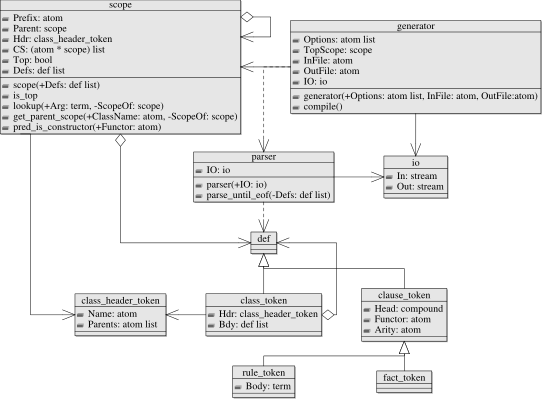
\includegraphics{./figs/uml.eps}
\caption{A UML class diagram for the compiler}
\label{fig:1}
\end{figure}

A simplified UML class diagram of the compiler is given in Figure~\ref{fig:1}. The \emph{generator} class has a constructor that takes an input file, output file, and a list of options. It contains a predicate, compile/0, that acts as the main entry point and compiles from OOPL to Prolog, its operation is described in section~\ref{sec:gen}. The \emph{parser} class performs lexing and parsing, and is covered in the Lexing and Parsing section.

\section{Lexing and Parsing}

Typically the first two stages in the front end of a compiler is lexing and parsing the input\cite{DRAGON}. The aim of these two steps is to first convert a stream of symbols into one of tokens, and then the token stream into a parse tree. There are many tools for automatically generating an efficient lexer/parser from a context-free grammar\footnote{e.g. LEX, YACC and similar tools} which would normally be employed at this point, however Prolog contains the inbuilt predicate `read_term/3' which handles most of this functionality.

\subsection{The read_term/3 Predicate}

The ISO standard\cite{ISOPROLOG} predicate read_term(+Stream, -Term, +Options) is true if and only if a Prolog term can be read from `Stream' and unified with `Term' controlled by the list of options `Options'. It reads until it encounters a dot character followed by whitespace, the sequence normally used to delimit a Prolog clause.

\bigskip

The term returned by read_term/3 is the same as if the characters read in had appeared in Prolog source, so escape characters are stripped away and character sequences starting with captial letters or underscores are read in as fresh variables. One important option is \emph{variable_names(Eqs)}: read_term/3 will unify the Eqs variable with a list of the form $[=(N_1, V_1), ..., =(N_n, V_n)]$ that associates the names N with variables V. This can be used to keep track of the original variable name.

\subsection{Declaring New Operators}

As OOPL is syntactically a strict superset of Prolog, to allow the read_term/3 predicate to correctly parse OOPL it suffices to declare new operators. This is done in Prolog with the op/3 predicate. The predicate op(+Precedence, +Type, :Name) takes a numeric precedence, a type (i.e. prefix, infix, postfix) and a name to register a new operator. From then on when the parser encounters the operator it will parse it as a Prolog term. e.g. after the directive:

\begin{verbatim}
:- op(100, yfx, ::).
\end{verbatim}

\noindent the string X::Y will then be read in as the term ::(X, Y), that is a compound of arity 2, with functor ::. For each of the operators added by OOPL (::, class, extends, endclass, private, public, static etc) an op directive was specified to allow the read_term/3 predicate to be used as a lexer/parser for OOPL.

\subsection{Parse Tree}

The read_term/3 predicate gives the parse tree for a single Prolog clause a compound term. This term is recursively wrapped to allow the compiler to disambiguate terms. Using variables as terms to represent syntactic variables was considered bad practice as they can unify with other arbitrary terms. Instead the atom used to name them in the source was used in the parse tree. This would mean however that the atom `X' and the variable X would then become indistinguishable. To remedy this the atom(`X') and var(`X') compounds are used. This means however that the compound var(`X') in the source would become indistinguishable from the variable X. This is why compounds are wrapped as well with `compound', so the compiler can tell if a compound was a part of the source program, or was performed by the parser. This also means the action of the compiler can be directed by pattern matching on the syntax of the tagging. For some term T:

\begin{itemize}
	\item{If T is an atom: return atom(T).}
	\item{If T is a compound: return compound(T') where T' is T with all its arguments tagged.}
	\item{If T is a named variable: return var(N) where N is the name of the variable.}
	\item{If T is an anonymous variable: return var(`_').}
\end{itemize}

\bigskip

The parser class repeatedly reads terms and warps them as above to build up a parse tree for the entire program. The constructor for the parser takes an IO object for the source file. The predicate parse_until_eof/1 unifies its argument with a list of def objects, see Figure~\ref{fig:1}, that represent the entire file. These objects are used as constructs in the compiler to represent the different tokens and associated values, and should not confused with objects the user defines. Each object is either a class_token or a clause_token (which are further separated into rule_token  and fact_token). The class_token object contains the list of def objects that appeared within a class in the source file. The class_header_token contains the name of the class and a list of the names of its parents.

\subsection{Working With Multiple Files}

To load plain Prolog files, SWI-Prolog provides two predicates: consult/1 and include/1. The predicate consult/1 can appear anywhere a goal would, and adds all the clauses in given file to the current database. The include/1 predicate can be used within a directive, and textually includes the target file in the program. As the simpler of the two, OOPl provides support for the directive oopl_include, e.g.:

\begin{lstlisting}
:- oopl_include(+file_path).
\end{lstlisting}

\noindent which is expanded by the lexer/parser, and acts in a similar way to Prolog's include/1 and textually includes the provided file before further compilation. It does this by creating a new instance of the parser class to recursively handle the new file, and appends the result into the list of def objects. Because of this the compiler's output is always a single file and partial recompilation is not possible, ideally an oopl_consult/1 predicate would also be added in the future which would handle files separately.

\section{Code Generation}
\label{sec:gen}
The second phase of the compiler is take the parse tree and output it in Prolog. For the most part this is relatively simple as OOPL is just an extension to Prolog so most of the language maps directly. The handling of the new features introduced by OOPL is discussed below.

\subsection{Scope Structure}

Throughout the compilation process information about the current scope and to find if and where certain things are defined is needed. For each scope (i.e. the top scope and every class's scope) we create an instance of the scope class\footnote{This is only required as a Compile-Time construct}. This class contains a constructor that takes the list of def objects produced by the parser and creates a recursive structure that provides many utility functions used by the compiler. 

\bigskip

The most important predicate it provides is lookup/2. The predicate lookup(+Arg, -ScopeOf) is true if and only if Arg is visible at the current scope, and ScopeOf can be unified with the scope where Arg is defined. Arg can be either be the compound pred(Name,N), to look up a predicate Name/N, or the compound class(Name), to look up a class called `Name', or field(Name) to look up a field called `Name'.The lookup predicate performs this search in the way defined in the preparation chapter, by first looking in the current class's scope, then up the chain of parent classes, and finally in the enclosing scope.

\subsection{Access}

The mechanism for accessing a member of an object is defined in a separate runtime library, see the runtime section. However, the compiler is required to replace the functional style :: operator with a predicate access/3. 

\bigskip

If a clause has an expression X::Y occurring anywhere within it we create a new temporary variable, T, and insert a new goal into a conjunction just before T is first needed. To avoid repeatedly accessing the same member, we use T for every occurrence of X::Y in the clause. For example, if we have a clause with a body of the form $A_1, ..., A_k, ..., A_n$ where $A_k$ is the first goal that contains the expression X::Y then we replace it with a body of the form $A_1, ..., access(X, Y, T), [T/X::Y]A_k, ..., [T/X::Y]A_n$. We recursively repeat this process (including on the new goal added to the conjunction) until every occurrence of :: has been removed. This can be done by scanning through the conjunction from left to right only once. We simply keep a set of  replacements that have already been made, and if we find another occurrence of the :: operator with the same arguments we can use the same replacement.

\bigskip

Another consideration is what to do if we find an occurrence of :: within the head of a clause. In this case we perform a similar replacement of the syntax with a new temporary, and we place the resulting goal as the first in the bodies conjunction. This can transform a fact into a rule. It is important that the new goal is evaluated before those in the body, as if it failed at the end of a body containing a cut it would give incorrect behavior.

\subsection{Fields}

Predicates within a class are allowed to pattern-match on fields. To provide this functionality, any time the compiler encounters a term of the form var(X) it first performs a lookup in the current scope, with an argument of field(X). If X is found to be a field, it replaces it with This::`X' and then falls back on the technique described in the Access subsection. Otherwise the definition of fields themselves cause no extra clauses to be generated.  

\subsection{Predicates}

In order to convert predicates within a class to Prolog predicates, two things occur. Firstly, the name of the predicate is mangled with the prefix of the current scope. This resolves conflicts if a predicate with the same name is defined in several scopes. Secondly, if the current scope is not the top scope, the implicit `This' argument is added to the predicate and its arity is increased by one. If the body of the predicate does not ever reference the `This' variable, the extra argument is made anonymous so further compilation steps do not raise any warnings.

\bigskip

In the case that a predicate defined in a child class is also defined in a parent class, an additional clause is inserted in order to implement the inheritance rules. For example, if class a is the parent of class b, and they both define foo/1 then we generate following rule for foo/2 (remembering to increase the arity by 1 for the `This' argument)

\begin{lstlisting}
b_foo(T1, T2) :- a_foo(T1, T2).
\end{lstlisting}

\noindent This clause is inserted after other b_foo clauses; this ensures that the programmer can use a cut to override behavior in the classical sense.

\bigskip

For every predicate that we encounter in the body of a clause we may need to its name to refer to the new predicate. For example, if we have some predicate, p/1, we can perform a lookup using the lookup predicate on the current scope object, with pred(p,1) as the argument. If this succeeds then we do one of two things:

\begin{itemize}
	\item if p is outside of a class: we simply rename p to refer to the mangled name.
	\item if p is inside of a class: we replace p with This::p.
\end{itemize}

The second transformation ensures that the predicate is resolved dynamically.

\subsection{New}

The `new `predicate, like the standard Prolog `call' predicate, has a variable number of arguments. There is no way of defining a predicate like this in Prolog, in fact SWI-Prolog has to deal with `call' specially in the compiler. This does mean, however, that `new' cannot be defined in the standard library for OOPL. Instead, it is decomposed into a combination of other predicates, including the call predicate which can then be compiled separately by SWI-Prolog. The syntax new(C, O, A1, ..., An) is first undergoes a macro like expansion into two new goals, using Prolog's `*-$>$' syntax.

\begin{lstlisting}
build_class(C, O),
(C::`Constructor' \= none) *-> 
	call(O, A1, ... An) ; 
	true
\end{lstlisting}

\noindent and then further compiled to remove the introduced/remaining non-Prolog syntax. The predicate build_class/2 is provided by the runtime (see below) and makes a new object with fresh variables for fields. The next expression adds the constructor as a goal. The `*-\textgreater' operator is a standard Prolog operator, and is roughly speaking `if then else'. The goal A *-\textgreater B ; C first attempts to satisfy A, it then cuts any choice points A may have created, and if it succeeded then B is added as a goal, otherwise C is.

\subsection{Classes}

For every class, say of name x, defined in the source two predicates are produced as output: class_def_x/1 and class_def_construct_x/1. These predicates will both unify their single argument with the object representing class x. They do this in two different ways however. class_def_construct_x is defined as follows:

\begin{lstlisting}
class_def_construct_x(X) :- class_def_classType(T), new(T, X, ...).
\end{lstlisting}

\noindent It first gets the class `classType' which is used to represent other classes, and then constructs a new instance of it, passing x's name, constructor, parents, predicates, fields, and outer class as arguments to classType's constructor (here written as `...' for brevity).

\bigskip

The classType constructor is defined in the runtime library and is tasked with building the objects to represent a class. Constructing the class this way means the implementation of objects can be kept separate from the compiler which only needs to know the interface to the `classType' constructor. The line above is not output verbatim, but is first further transformed to remove the `new' keyword. In order to avoid creating multiple instances of the x class, which would increase the memory footprint of objects, we do not make calls to this predicate directly. Instead a directive is inserted into the source file:

\begin{lstlisting}
 :- class_def_construct_x(X), nb_setvar(x, X).
\end{lstlisting}
 
   
\noindent Prolog has support for global variables. Two predicates for manipulating global vairables are nb_setvar and nb_getvar, which set and get variables respectively. The directive above creates a global variable that is bound to the object representing class x, and can be accessed using its name. class_def_x/1 is used to retrieve this instance:

\begin{lstlisting}
 class_def_x(X) :- nb_getvar(x, X).
\end{lstlisting}
 
\noindent Recall that in section~\ref{sec:lang} we said that atoms with the same name and in the same scope as a class should not be atoms, but rather should refer to the class. During compilation, for every atom we encounter, we have to check if it refers to a class. We verify this by invoking the lookup predicate on the current scope with class(x) as an argument. If x was a class in the current scope, we first add an extra goal class_def_x(T) to the current clause, in a similar fashion to how we lifted out the `::' syntax, where `T' is a new temporary variable, and then replace all occurrences of the atom `x' in the clause with the variable `T'.

\section{Runtime}

This section concerns the runtime representation of objects and their manipulation.

	\subsection{The OOPL Runtime}

The details of the representation of objects is made opaque to the compiler and programmer, and is performed by a small runtime library. The compiler inserts into its output a directive to include the runtime. The runtime library itself is written in OOPL (called standard.oopl) and contains:

\begin{itemize}
	\item The class that represents classes, classType.
	\item The predicate for building an uninitialised object, build_class/2.
	\item The predicate access/3 (called ::/3 in the source).
	\item A number of useful predicates for the programmer, such as object/1 and classof/2.
\end{itemize}

The first three are all used by code generated by the compiler. The other two are for use by the programmer. In a similar way that predicates are generated for other classes by the compiler, the runtime defines the classType class using a predicate class_def_classType. The predicate build_class(+Class, -Instance) takes a class and gives back an instance of that class, with all fields instantiated to fresh variables. The exact structure my implementation gives is detailed below. The implementation of access/3 depends on this structure and so it is also described below. Much like the predicates in standard Prolog atom/1, var/1, number/1, etc. that the programmer can use to inspect the type of terms at runtime, object/1(+O) is true if and only if O is an object. The predicate classof(+O,?C) is true if and only if the class of O is C, and can be used to perform reflection on classes.

	\subsection{Explicit Object Structure}
	
Objects were built using a Prolog compound, class(C,M), where C is the object's class, and M a structure which holds an object's members. This gives the correct unification behaviour of objects, as they will unify with other objects only when they share the same class and their members can be unified. Due to the way class objects are created and retrieved, even though every object contains its class the class itself is not duplicated, this means the memory cost of C is that of a single pointer. For the M structure itself, two approaches were taken and are detailed below.
	
		\subsubsection{Simple Structure}
		
Initially a very simple structure was used in order to get the project working as quickly as possible and allow bootstrapping. The `M' structure was itself a compound, it had the functor `members' and arity equal to the number of members an object had. Each argument in the compound was a tuple of the form (Key, Value), and the access predicate would employ a linear search to look for a member. Both predicates and fields were included in the compound, in no particular order. This made the access/3 predicate very simple as Prolog provides the arg/3 predicate to find the Nth argument of a term. Although simple and lightweight, this meant that the performance of objects suffered as they grew larger, and every object would unnecessarily keep a copy of the predicates it contained.

		\subsubsection{Complex Structure}
		
In an attempt to make access more efficient, and to reduce the size of objects, a second structure was created. Instead of searching through a compound in linear time, a hash table was used for the `M' structure, and furthermore it only contained fields. The implementation of the hash table is discussed below. As the object now only contained fields, the access/3 predicate is made slightly more complex and has to make several lookups. First a lookup in M is made to see if the desired member is a field. Failing that, the class of the object is retrieved using classof/2, and a recursive field lookup is made to find the predicates belonging to the class. Finally a lookup in the predicates is made, and the result closed with a copy of the object in order to provide the implicit `This' argument. This added quite a lot of overhead to dispatch, as several calls were required, in including several hash function calls. The cost of this is covered in the evaluation.
		
		\subsubsection{A Prolog Hash Table}

In order to support the lookup of fields and predicates in constant-time it was required to design a hash table in Prolog that supported insertion and lookup operations. The insert/2 predicate takes a table and a key-value pair and adds it to the table. The lookup/2 predicate also takes a table and key-value pair, but its behaviour depends on the provided key. If a lookup is performed on the pair (K, V) in the table then:

\begin{itemize}
	\item if K is a variable: (K, V) is successively unified with every pair.
	\item if K is an atom: if K is not a key in the table, then fail, otherwise attempt to unify V with the value stored in the entry.
\end{itemize}

In this way the lookup predicate acts as both a get and set, although it cannot change any particular entry, only further unify the value associated with a key. Upon backtracking any changes made to the table are undone. The implementation of the table, and the method for performing a lookup is given bellow.

\bigskip

\begin{figure}
 \centering
\includegraphics{./figs/hash2.eps}
\caption{Looking up a key that is an atom.}
\label{fig:2}
\end{figure}
\begin{figure}
 \centering
\includegraphics{./figs/hash3.eps}
\caption{Looking up a key that is an atom and finding the wrong key.}
\label{fig:3}
\end{figure}
\begin{figure}
 \centering
\includegraphics{./figs/hash4.eps}
\caption{Looking up an atomic key that isn't in the table.}
\label{fig:4}
\end{figure}
\begin{figure}
 \centering
\includegraphics{./figs/hash1.eps}
\caption{Looking up a key that is a variable.}
\label{fig:5}
\end{figure}

The table itself is the compound `table(S, T)', here S is an atom that records the size of the table, and T a compound with arity equal to S, whose arguments are the table's entries. A strategy of Open Addressing with strobe size 1 was employed. If an atomic key is provided it is hashed and used as an initial index into the table. If an entry is found at that index with the correct key, as in Figure~\ref{fig:2}, the provided value is unified with the value found in the table. In Figure~\ref{fig:2} this would result in the unification X=2. If there is a key there, but not the correct one (as in Figure~\ref{fig:3}), the next index is tried in the same way. Finally, if an entry is found with the key unbound like in Figure~\ref{fig:4}, then the key is not in the table and we fail. If the key provided is a variable like in Figure~\ref{fig:5}, then a linear search pattern is used, and skipping any entries that have unbound keys, we attempt to unify the provided pair with every pair in the table. In Figure~\ref{fig:5} this would result in X=a, and then upon backtracking X=c. Note that the performance of the table is not guaranteed to be constant time, in the worst case where every key hashes to the same value we will see lookup times proportional to the number of entries in the table. However, if we make the table sparse enough and use a hash function that will distribute entries uniformly the number of entries we have to step is expected to be constant. 

\bigskip

Insertion is very similar to a lookup, but instead of failing when we reach an empty entry we unify the entry with the new key-value pair. Furthermore, the key must be a value and not already be in the table. Insertion into the table is only performed by the runtime, when an object is constructed, and so there is no chance of the table raising an exception due to a user program. 

\bigskip

Using field names as keys to the table, this provides a basis for the semantics we require for accessing members. If we provide an unbound variable then we get every field-value pair, and if we provide a field name we get just the correct value, but now in constant time. The number of fields an object has is constant (it is defined by its class), so we can choose an appropriate size for a hash table when we construct the object.

	\subsection{Representing Classes}
	
As previously mentioned, classes are embodied by objects at runtime that are instances of a special class called classType. The class called `classType' is defined in OOPL as:

\begin{lstlisting}
class classType.

	% The fields that store all the class information.
	Name.
	Fields.
	Predicates.
	Parent.
	Outer.
	Constructor.
	
	% The constructor simply unifies its arguments
	% with the fields. There is no need to use the
	% `=' operator.
	
	classType(Name, 
		Fields,
		Predicates,
		Parent,
		Outer,
		Constructor).
endclass.
\end{lstlisting}

\noindent Every class in OOPL is represented at runtime by an instance `classType', including the class `classType' itself! As every object contains its class, this would mean that objects become cyclic as the class of classType is itself. This cycle would cause all objects to fail the occurs check. To remedy this we use the atom `self' instead of an argument which would lead to in infinite cycle. For example, instead of writing:

\begin{lstlisting}
X = (X, Y)
\end{lstlisting}
\noindent write:
\begin{lstlisting}
X = (self, Y)
\end{lstlisting}

\noindent This makes the explicit structure of objects finite. However, in order to make it appear infinite to the programmer (as is expected) the classof/2 predicate in the runtime library automatically substitutes the atom `self' for the object containing it. Some pseudocode for the classof/2 predicate:


\begin{lstlisting}
 classof((X,Y), Z) :- IF X = self THEN Z = (X,Y) ELSE Z = X.
\end{lstlisting} 

\noindent As the programmer should never explicitly manipulate objects, using `self' to remove cycles should not change any other functionality. 

\section{Bootstrapping}

As the project progressed and more features were added to the compiler, a succession of snapshots of a compiled version of the compiler, as well as the runtime library, were made to restart the bootstrapping process. Whenever there was a need to compile the source for a new version of the compiler the following steps were performed:

\begin{center}
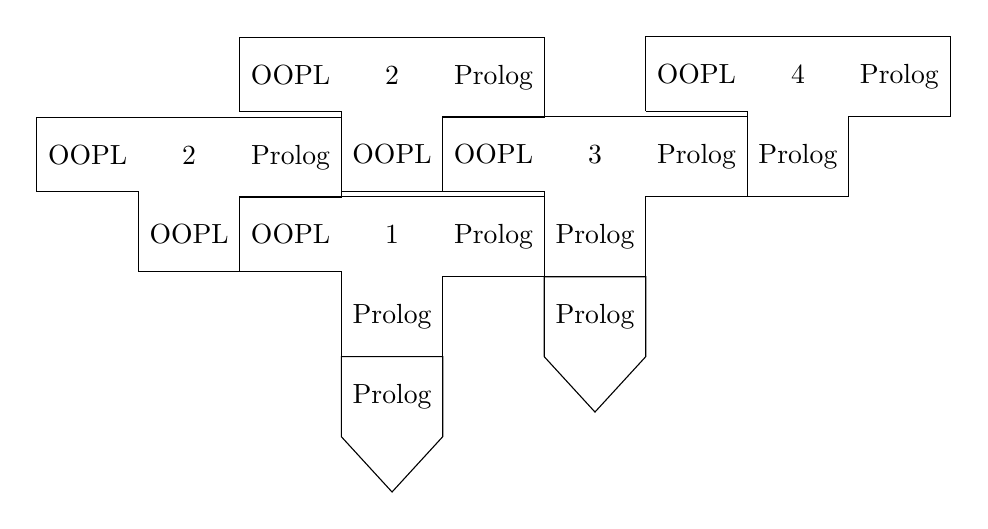
\begin{tikzpicture}
	\node(compiler1) [tblock] {\tblocktextnm{OOPL}{Prolog}{Prolog}{1}};
	\tblockoutline{compiler1};
	
	\node(compiler2) at (compiler1-1-1.north west) [tblock, anchor = compiler2-2-2.north east] {\tblocktextnm{OOPL}{Prolog}{OOPL}{2}};
	\tblockoutline{compiler2};
	
	\node(compiler3) at (compiler1-1-3.north east) [tblock, anchor = compiler3-2-2.north west] {\tblocktextnm{OOPL}{Prolog}{Prolog}{3}};
	\tblockoutline{compiler3};
	
	\node(compiler4) at (compiler3-1-1.north west) [tblock, anchor = compiler4-2-2.north east] {\tblocktextnm{OOPL}{Prolog}{OOPL}{2}};
	\tblockoutline{compiler4};
	
	\node(compiler5) at (compiler3-1-3.north east) [tblock, anchor = compiler5-2-2.north west] {\tblocktextnm{OOPL}{Prolog}{Prolog}{4}};
	\tblockoutline{compiler5};
	
	\wsupt{Prolog}{compiler1};
	\wsupt{Prolog}{compiler3};
\end{tikzpicture}
\end{center}

First the new version of the compiler, 2, was compiled using the snapshot, 1. This gave a compiler, 3, that had the new feature. However, it itself would be unable to use the feature, so to fix this we run 3 on 2 to get 4 which both supports the new feature and uses it. At this point further iterations of the bootstrapping process only served to verify the fixed point had been reached. If the feature is later relied on in the compiler, the snapshot 1 is replaced by 4 to avoid having to create an unnecessarily long chain of bootstrapping steps when recovering from a problem, or cloning the project on a new machine.

\section{Interpreter}

As with Prolog programs, users expect to be able to submit queries to a OOPL program. In order to interface with the output produced at the compile step and still be able to use new syntax, such as new and ::, an interactive interpreter is required. At the end of the programs clauses the compiler inserts a directive to ensure the interpreter is loaded and an entry point goal is automatically invoked. The compiler also outputs a new fact, defined_names/1, at the end of the output source file which contains the names of all classes and predicates defined at the top level.

\bigskip

The interpreter works on the principle of a \emph{read-evaluate-print loop}(REPL). The user provides a single query, this query is then evaluated (in this case transformed from OOPL into Prolog and then passed on to the underlying Prolog interpreter) and the resulting variable bindings, or exceptions, are printed out to the console as usual. This process then repeats. The work of reading and evaluating the input is a very similar task to that performed by the compiler. The interpreter itself is also written in OOPL, and so can make use of inheritance to extend functionality of the compiler. The interpreter class simply extends that of the generator, slightly modifying behavior to call the result rather output it to a file. The parser class is also extended to not replace variables with atoms, as they are required for evaluation not printing. Finally the scope class is extended to use the defined_names/1 predicate to rebuild the top level scope object that the compiler created. This is required to map the original predicate names and class names to the predicates produced by the compiler.

\section{Unit Testing}

SWI-Prolog offers a powerful framework for writing unit tests in Prolog. A single predicate offered a fine-grained level of testing, and so tests were designed for most of the important predicates within the compiler. As the unit test framework only works with Prolog, not OOPL, some modification was required. This was done by using the OOPL interpreter to execute all the queries in the unit test module. The `show_coverage/1' predicate takes a goal, in this case the entry point for the unit tests, and shows the percentage of clauses that are entered, and the percentage that only ever failed. The results of a run of the unit tests are given below:
 
 \begin{verbatim}
 ?- test.
% PL-Unit: bootstrap .. done
% PL-Unit: utils ...... done
% PL-Unit: parse ..... done
% PL-Unit: generate . done
% All 14 tests passed
==============================================================================
                               Coverage by File                               
==============================================================================
File                                                     Clauses    %Cov %Fail
==============================================================================
...ood/desktop/uni/20142015/project/src/utils/utils.pl        29    93.1   0.0
...p/uni/20142015/project/src/make_prolog_interface.pl         2   100.0   0.0
...ood/desktop/uni/20142015/project/build/interpret.pl       210    80.0   4.3
.../desktop/uni/20142015/project/build/standard.out.pl        13    61.5   0.0
...wood/desktop/uni/20142015/project/build/generate.pl       174    88.5   5.2
==============================================================================
 \end{verbatim}

Many of the input files have been combined into the last entry, this is due to the compiler only producing a single output file and the tests operating on that rather than the source.

\chapter{Evaluation}

The focus of this chapter is to evaluate the results of the project, as well as the steps taken to achieving them. The functionality and performance of the output produced by the compiler is evaluated here, and its output is compared to that of standard Prolog and the Logtalk implementation of Prolog-with-Objects. Finally an evaluation of the bootstrapping process is given as well as a commentary on the difficulties it created.

\section{Correctness}

The primary concern of the project is that the compiler produces output which obeys the semantics outlined in the Preparation section. A number of code examples were carefully crafted that exemplified each feature of the language, and their outputs were compared with the expected result. The features under test are all those in Section~\ref{sec:req} under `must'.

\subsection{Examples}

Each of the examples below contains both the OOPL source (on the left of each table), and the results of a number of queries (on the right of each table) to the OOPL interpreter. The Objects themselves are pretty printed in a tree like structure. The `?-' prompt  is for a query, and the `\textbar:' prompt for a single character. The interpreter will print `true' followed by the variable bindings for every success, and `fail' when there are no more.

	\subsubsection{Constructing Classes}
This example shows how a class can be declared with a constructor, and the `new' predicate used to build an instance. It specifically illustrates how multiple constructors can be declared, and how backtracking occurs over `new'. There is a single class called \emph{construct}, which has two constructors \emph{construct/3} and  \emph{construct/2}.  The \emph{construct/3} constructor predicate has two definitions, the second reverses the order of the arguments. When we retry the goal, we should try the other constructor to get the fields assigned to differently. The  \emph{construct/2} constructor does more than just assign its arguments, it makes the third field the sum of the other two.
	
\definecolor{llightgray}{rgb}{.9,.9,.9}
\definecolor{lightgray}{rgb}{.8,.8,.8}

\newsavebox{\boxaa}
\setbox\boxaa\hbox{
\begin{minipage}{0.5\hsize}
\begin{lstlisting}
?-new(construct, C, a, b, c).
\end{lstlisting}
\begin{lstlisting}[backgroundcolor=\color{lightgray}]
true.
C = instance of construct.
        |
        |-Field1=a.
        |-Field2=b.
        |-Field3=c.
|:
\end{lstlisting}
\begin{lstlisting}[backgroundcolor=\color{llightgray}]
true.
C = instance of construct.
        |
        |-Field1=c.
        |-Field2=b.
        |-Field3=a.
|:
\end{lstlisting} 
\begin{lstlisting}[backgroundcolor=\color{lightgray}]
fail.
\end{lstlisting}
\end{minipage}
}

\newsavebox{\boxab}
\setbox\boxab\hbox{
\begin{minipage}{0.5\hsize}
\begin{lstlisting}
?-new(construct, C, 1, 2).
\end{lstlisting}
\begin{lstlisting}[backgroundcolor=\color{lightgray}]
true.
C = instance of construct.
        |
        |-Field1=1.
        |-Field2=2.
        |-Field3=3.
|:
\end{lstlisting}
\begin{lstlisting}[backgroundcolor=\color{llightgray}]
fail.
\end{lstlisting}
\end{minipage}
}

\begin{center}
\begin{tabular}{c|l}
	Source & Command Line Input/Output \\
	\hline
	\small
\begin{lstlisting}
class construct.

  Field1. Field2. Field3.

		
  construct(Field1,
            Field2, 
            Field3).
  
  construct(Field3,
            Field2,
            Field1).


  construct(Field1,
            Field2) :-
    Field3 is Field1 + Field2.
    
endclass.
\end{lstlisting}

&

\begin{minipage}{0.5\hsize}
\vspace*{1ex}
\fbox{\usebox{\boxaa}}

\fbox{\usebox{\boxab}}
\end{minipage}

\\
\end{tabular}
\end{center}

\noindent The first query shows how backtracking over constructors works. It succeeds twice, first correctly initialising all three fields, then backtracking and using the second constructor. The second query shows how using a different number of arguments calls the correct constructor, it succeeds only once as there is only one construct/2 predicate, but also performs the sum as expected.

	\subsubsection{Accessing Members}
	
This example shows the use of the `::' operator to access both fields and member predicates. There is a single class, \emph{members}, that has three fields (automatically unified with the numbers `1', `2' and `4' when the object is constructed) and two predicates: one which returns the sum of its fields, the other the product.
	
	
\newsavebox{\boxba}
\setbox\boxba\hbox{
\begin{minipage}{0.5\hsize}
\begin{lstlisting}
?-new(members, M),
  (F1, F2, F3) = 
    (M::`Field1',
     M::`Field2',
     M::`Field3'),
  call(M::predicate1, X1),
  call(M::predicate2, X2).
\end{lstlisting}
\begin{lstlisting}[backgroundcolor=\color{lightgray}]
true.
M = instance of members.
        |
        |-Field1=1.
        |-Field2=2.
        |-Field3=4.
F1=1.
F2=2.
F3=4.
X1=7.
X2=8.
\end{lstlisting}
\end{minipage}
}	


	
	\begin{center}
\begin{tabular}{c|c}
Source & Command Line Input/Output \\
\hline
	\small
\begin{lstlisting}
class members.

  Field1. Field2. Field3.
  
  
  members :-
    Field1 = 1,
    Field2 = 2,
    Field3 = 4.


  predicate1(X) :-
    X is Field1 + Field2 + Field3.
    
  predicate2(X) :-
    X is Field1 * Field2 * Field3.
    
endclass.
\end{lstlisting}
&

\begin{minipage}{0.5\hsize}
\vspace*{1ex}
\fbox{\usebox{\boxba}}
\end{minipage}

\\
\end{tabular}
\end{center}

\noindent The query first constructs an instance of  \emph{members}, and unifies F1, F2, and F3 with Field1, Field2 and Field3 respectively. Two calls are also made, the first to predicate1 and the second to predicate2. X1 and X2 are unified with the sum and product respectively.

	\subsubsection{Scoping}
	
This example shows how predicates resolve differently depending on the scope. We define a predicate \emph{predicate/1} in several different places. There are 4 classes, `a' through `d', each has a constructor that calls predicate/1, which resolves differently in each case.

\newsavebox{\boxca}
\setbox\boxca\hbox{
\begin{minipage}{0.5\hsize}
\begin{lstlisting}
?-predicate(X).
\end{lstlisting}
\begin{lstlisting}[backgroundcolor=\color{lightgray}]
true.
X=outside.
|:
\end{lstlisting}
\end{minipage}
}	

\newsavebox{\boxcb}
\setbox\boxcb\hbox{
\begin{minipage}{0.5\hsize}
\begin{lstlisting}
?-new(a, _, X).
\end{lstlisting}
\begin{lstlisting}[backgroundcolor=\color{lightgray}]
true.
X=within_a.
|:
\end{lstlisting}
\end{minipage}
}	

\newsavebox{\boxcc}
\setbox\boxcc\hbox{
\begin{minipage}{0.5\hsize}
\begin{lstlisting}
?-new(b, _, X).
\end{lstlisting}
\begin{lstlisting}[backgroundcolor=\color{lightgray}]
true.
X=within_a.
|:
\end{lstlisting}
\end{minipage}
}	

\newsavebox{\boxcd}
\setbox\boxcd\hbox{
\begin{minipage}{0.5\hsize}
\begin{lstlisting}
?-new(c, _, X).
\end{lstlisting}
\begin{lstlisting}[backgroundcolor=\color{lightgray}]
true.
X=within_c.
|:
\end{lstlisting}
\end{minipage}
}	

\newsavebox{\boxce}
\setbox\boxce\hbox{
\begin{minipage}{0.5\hsize}
\begin{lstlisting}
?-new(d, _, X).
\end{lstlisting}
\begin{lstlisting}[backgroundcolor=\color{lightgray}]
true.
X=outside.
\end{lstlisting}
\end{minipage}
}	

	\begin{center}
\begin{tabular}{c|c}
Source & Command Line Input/Output \\
\hline
	\small
\begin{lstlisting}
predicate(outside).

class a.
  predicate(within_a).
  a(X) :- predicate(X).
endclass.

class b extends a.
  foo(X) :- predicate(X).
  b(X) :- predicate(X).
endclass.

class c extends a.
  predicate(within_c).
  c(X) :- predicate(X).
endclass.

class d.
  d(X) :- predicate(X).
endclass.
\end{lstlisting}
&
\begin{minipage}{0.5\hsize}
\vspace*{1ex}
\fbox{\usebox{\boxca}}
\fbox{\usebox{\boxcb}}
\fbox{\usebox{\boxcc}}
\fbox{\usebox{\boxcd}}
\fbox{\usebox{\boxce}}
\end{minipage}
\\
\end{tabular}
\end{center}

Five queries were executed. The first calls `predicate' at the top level. The other four construct each class in order. With class `a' we get `within_a' as a result. With class `b' we get `within_a' as `b' extends `a'. With class `c' we get a `within_c' as although it also extends `a', it also has a definition of `predicate'. Finally for `d' we resolve the predicate to the top level definition, outside all the classes as `d' has neither its own definition nor does it inherit one.

\subsubsection{Inheritance}
	
This example shows how inheritance extends behavior on backtracking. There are four classes, each with a predicate \emph{f/1}. The class `class_d' extends `class_b' extends `class_a', as well `class_c' extends `class_a'.


\newsavebox{\boxda}
\setbox\boxda\hbox{
\begin{minipage}{0.52\hsize}
\begin{lstlisting}
?-new(class_a, X), call(X::f, Y).
\end{lstlisting}
\begin{lstlisting}[backgroundcolor=\color{lightgray}, belowskip=0pt]
true.
X = instance of class_a
Y=a.
|:
\end{lstlisting}
\begin{lstlisting}[backgroundcolor=\color{llightgray}, belowskip=0pt]
fail.
\end{lstlisting}
\end{minipage}
}

\newsavebox{\boxdb}
\setbox\boxdb\hbox{
\begin{minipage}{0.52\hsize}
\begin{lstlisting}
?-new(class_b, X), call(X::f, Y).
\end{lstlisting}
\begin{lstlisting}[backgroundcolor=\color{lightgray}, belowskip=0pt]
true.
X = instance of class_b
Y=b.
|: 
\end{lstlisting}
\begin{lstlisting}[backgroundcolor=\color{llightgray}, belowskip=0pt]
true.
X = instance of class_b
Y=a.
|: 
\end{lstlisting}
\begin{lstlisting}[backgroundcolor=\color{lightgray}, belowskip=0pt]
fail.
\end{lstlisting}
\end{minipage}
}

\newsavebox{\boxdc}
\setbox\boxdc\hbox{
\begin{minipage}{0.52\hsize}
\begin{lstlisting}
?-new(class_c, X), call(X::f, Y).
\end{lstlisting}
\begin{lstlisting}[backgroundcolor=\color{lightgray}, belowskip=0pt]
true.
X = instance of class_c
Y=c.
|: 
\end{lstlisting}
\begin{lstlisting}[backgroundcolor=\color{llightgray}, belowskip=0pt]
fail. 
\end{lstlisting}
\end{minipage}
}

\newsavebox{\boxdd}
\setbox\boxdd\hbox{
\begin{minipage}{0.52\hsize}
\begin{lstlisting}
?-new(class_d, X), call(X::f, Y).
\end{lstlisting}
\begin{lstlisting}[backgroundcolor=\color{lightgray}, belowskip=0pt]
true.
X = instance of class_d
Y=d.
|: 
\end{lstlisting}
\begin{lstlisting}[backgroundcolor=\color{llightgray}, belowskip=0pt]
true.
X = instance of class_d
Y=b.
|: 
\end{lstlisting}
\begin{lstlisting}[backgroundcolor=\color{lightgray}, belowskip=0pt]
true.
X = instance of class_d
Y=a.
|: 
\end{lstlisting}
\begin{lstlisting}[backgroundcolor=\color{llightgray}, belowskip=0pt]
fail.
\end{lstlisting}
\end{minipage}
}

\begin{adjustwidth}{-0cm}{-0cm}
\begin{center}
\begin{tabular}{c|c}
Source & Command Line Input/Output \\
\hline
	\small
\begin{lstlisting}
class class_a.

  f(a).
  
endclass.


class class_b extends class_a.

  f(b).
  
endclass.


class class_c extends class_a.

  f(c) :- !.
  
endclass.


class class_d extends class_b.

  f(d).
  
endclass.
\end{lstlisting}
&
\begin{minipage}{0.5\hsize}
\vspace*{1ex}
\fbox{\usebox{\boxda}}
\fbox{\usebox{\boxdb}}
\fbox{\usebox{\boxdc}}
\fbox{\usebox{\boxdd}}
\end{minipage}
\\
\end{tabular}
\end{center}
\end{adjustwidth}

The first query constructs a class_a and calls f, getting `a' as a result. The second query constructs a class_b, when we call f we first get `b', but on backtracking get an `a' due to inheritance. With the third query we insert a cut, so even though class_c extends class_a we only get `c' as a result. Finally the last query shows this works with a larger hierarchy of inheritance, we get the sequence of solutions `d', `b', `a'. 

	\subsubsection {Dynamic Dispatch}
	
This example shows how the late binding and dynamic dispatch of predicates works in OOPL. We define a superclass called animal. It contains a predicate abstract predicate says/1, and a predicate vocalise/1 that will write to user_output any result of the says/1 predicate. The classes bird and polly all have animal somewhere in their class hierarchy, and define more clauses for says/1 so that when vocalise/1 is called we get different results.

\newsavebox{\boxea}
\setbox\boxea\hbox{
\begin{minipage}{0.50\hsize}
\begin{lstlisting}
?-new(bird, X), 
	call(X::vocalise).
\end{lstlisting}
\begin{lstlisting}[backgroundcolor=\color{lightgray}]
cheep cheep
true.
X = instance of bird
|: 
\end{lstlisting}
\begin{lstlisting}[backgroundcolor=\color{llightgray}]
fail.
\end{lstlisting}
\end{minipage}
}

\newsavebox{\boxeb}
\setbox\boxeb\hbox{
\begin{minipage}{0.50\hsize}
\begin{lstlisting}
?-new(polly, X),
	call(X::vocalise).
\end{lstlisting}
\begin{lstlisting}[backgroundcolor=\color{lightgray}]
Who's a pretty boy then?
true.
X = instance of polly
|: 
\end{lstlisting}
\begin{lstlisting}[backgroundcolor=\color{llightgray}]
cheep cheep
true.
X = instance of polly
|: 
\end{lstlisting}
\begin{lstlisting}[backgroundcolor=\color{lightgray}]
fail.
\end{lstlisting}
\end{minipage}
}

\begin{center}
\begin{tabular}{c|c}
Source & Command Line Input/Output \\
\hline
	\small
\begin{lstlisting}
class animal.
  
  % This is how we create
  % an abstract method.
  says(_) :- fail. 

  vocalise :-
    says(X),
    write(X),
    nl.
    
endclass.

class bird extends animal.
  says('cheep cheep').
endclass.

class polly extends bird.
  says(`Who\'s a pretty boy then?').
endclass.
\end{lstlisting}
&
\begin{minipage}{0.5\hsize}
\vspace*{1ex}
\fbox{\usebox{\boxea}}
\fbox{\usebox{\boxeb}}
\end{minipage}
\\
\end{tabular}
\end{center}

When we construct a bird and call vocalise, we get vocalise as defined in animal (as bird does not define its own), but the says definition of bird is used instead. Similarly for a new polly, we get the result of says from the polly class (and also the result from bird on backtracking, due to the behaviour of inheritance). 

	\subsubsection{Higher-Order Classes}
	
This final example shows how classes are teated as first-class citizens. There are only two classes, `a' and `b', and neither have any members.

\newsavebox{\boxfa}
\setbox\boxfa\hbox{
\begin{minipage}{0.50\hsize}
\begin{lstlisting}
?-member(Class, [a,b]), 
	new(Class, Object).
\end{lstlisting}
\begin{lstlisting}[backgroundcolor=\color{lightgray}]
true.
Class = instance of classType.
        |
        |-Name=a.
        |-Fields=[].
        |-Predicates=[].
        |-Parent=none.
        |-Outer=none.
        |-Constructor=none.
Object = instance of a
|: 
\end{lstlisting}
\begin{lstlisting}[backgroundcolor=\color{llightgray}]
true.
Class = instance of classType.
        |
        |-Name=b.
        |-Fields=[].
        |-Predicates=[].
        |-Parent=none.
        |-Outer=none.
        |-Constructor=none.
Object = instance of b
|: 
\end{lstlisting}
\begin{lstlisting}[backgroundcolor=\color{lightgray}]
fail.
\end{lstlisting}
\end{minipage}
}

	\begin{center}
\begin{tabular}{c|c}
Source & Command Line Input/Output \\
\hline
	\small
\begin{lstlisting}
class a.
endclass.

class b.
endclass.
\end{lstlisting}
&
\begin{minipage}{0.5\hsize}
\vspace*{1ex}
\fbox{\usebox{\boxfa}}
\end{minipage}
\\
\end{tabular}
\end{center}

We execute the query the binds the variable class to either a or b, using the member predicate, and then construct a new instance of it. In the first solution Class is bound to a, and so Object becomes a new instance of a. Class itself is an object of class classType that describes a. On backtracking we get the other solution, where Class is b.

\subsection{Incomplete Features}

Due to time constraints extensions to provide private/public/static predicates, multiple inheritance and inner classes were never completed. However they were partially completed in that the parser can handle everything but multiple inheritance, and most of the infrastructure was created in the generator to support multiple inheritance and inner classes.

\section{Performance}

The aim of extending Prolog with objects was to provide more expressiveness to the programmer, however this does incur a penalty in terms of execution time and memory overhead. This section quantifies these penalties and contrasts with other implementations. All tests were run on my own machine, running Windows 7, with an Intel i5-2500k CPU @3.3Ghz, using SWI-Prolog as the back-end compiler, version 7.1.33.

\subsection{Dynamic Dispatch}

In order to implement polymorphism within OOPL, predicate calls are all late bound and the cost of both looking the predicate up and calling it incurs an overhead. To quantify this the time to make a million calls was measured. As a comparison the times to call the \emph{Baseline} (the time it takes to call a normal Prolog predicate), and the \emph{Call Predicate} (the time to invoke using the inbuilt call/2 predicate) were also recorded. In order to measure the impact of having larger classes (and thus a greater search-space) a number of classes were defined, each with a larger number of predicates. In order to evaluate the pros of cons of the different object structures, both implementations were timed.

\begin{center}
\begin{tabular}{c|c|c}
Type of Call & \multicolumn{2}{c}{Time for 1 000 000 calls /s} \\
\hline
Baseline&\multicolumn{2}{c}{0.125}\\
Call Predicate&\multicolumn{2}{c}{0.203}\\
\hline
Dynamic Dispatch& Simple Structure & Complex Structure \\
\hline		
1 Member	&	0.39	&	2.92	\\
2 Members	&	0.343	&	2.93	\\
4 Members	&	0.53	&	2.93	\\
8 Members	&	0.702	&	2.9	\\
16 Members	&	1.05	&	2.93	\\
32 Members	&	1.72	&	2.89	\\
64 Members	&	3.04	&	2.93	\\
128 Members	&	5.71	&	2.93	\\
256 Members	&	11.1	&	2.93	\\
512 Members	&	21.8	&	2.96	\\
1024 Members	&	43.5	&	2.95	\\


\end{tabular}
\end{center}

As expected the time to make a call with the compound structure scaled roughly linearly with the number of members an object had, while the hash structure remained roughly constant although the extra cost of multiple calls to calculate the hash led to making it an order of magnitude slower for very small classes. Even for the simple structure with only a few, we are roughly incurring a 3-4x slowdown when making calls. For an imperative language where calls only make up a small part of the total execution time (we tend to make heavier use of if blocks and loops for flow control), this may not be too significant. However, Prolog relies heavily on making calls and this slowdown may prove to be significant. There do exist solutions to this problem, such as inline caching to remove the lookup and runtime inlining to remove the call entirely, but this was considered outside the scope of the project. The actual cost to an example program is explored later with a comparison example.

\subsection{Objects}

Due to the way objects are used in OOPL, their creation and destruction (via garbage collection) is commonplace. Here we evaluate the how much time and space is required to allocate an object and to call a simple constructor. Garbage collection was forced before and after the test. The same classes from the Dynamic Dispatch benchmarks were used, with a constructor with no arguments and having an empty body.

\subsubsection{Time}

The time to construct and destroy one hundred thousand objects were recorded. The work for construction is the allocation of memory, creation of all relevant structures and lookup/invocation of the constructor. Again we compare the use of both object structures.

\begin{center}
\begin{tabular}{c|c|c}

& \multicolumn{2}{c}{Time for 100 000 constructions /s} \\
\hline
Number of Predicates & Simple Structure & Complex Structure \\
\hline
1	&	0.281		&	0.514	\\
2	&	0.328		&	0.53	\\
4	&	0.421		&	0.421	\\
8	&	0.608		&	0.53	\\
16	&	0.967		&	0.53	\\
32	&	1.68		&	0.53	\\
64	&	3.14		&	0.515	\\
128	&	6.04		&	0.53	\\
256	&	11.8		&	0.515	\\
512	&	23.3		&	0.53	\\
1024	&	46.6		&	0.515	\\


\end{tabular}
\end{center}

The simpler structure naively keeps a copy of all the classes predicates, this gives the linear scaling with the number of predicates the class has. The Complex Structure avoids this and so does everything in constant time.

\subsubsection{Space}

SWI-Prolog maintains 3 stacks for memory allocation: a local stack for storing calls, a global stack to store terms, and a trail stack to store assignments. The objects created by `new' live on the global stack. Again using the same classes with differing numbers of predicates, the footprint on the global stack for a single object was measured.

\begin{center}
\begin{tabular}{c|c|c}

& \multicolumn{2}{c}{Global Stack Footprint of One Object /bytes} \\
\hline
Number of Predicates & Simple Structure & Complex Structure \\
\hline
1		&	88		&	56	\\
2		&	136		&	56	\\
4		&	232		&	56	\\
8		&	424		&	56	\\
16		&	808		&	56	\\
32		&	1576	&	56	\\
64		&	3112	&	56	\\
128		&	6184	&	56	\\
256		&	12328	&	56	\\
512		&	24616	&	56	\\
1024	&	49192	&	56	\\


\end{tabular}
\end{center}

\noindent Again due to the simple structure keeping a copy of every predicate, the objects get larger the more predicates are added. The complex structure, however, stays constant as it simply keeps a reference to a common class object. Objects have a relatively large memory footprint as compared to implementations in other languages\footnote{e.g. Java HotSpot VM will use only 8 bytes for a header, and either 4 or 8 bytes for each reference depending on 32 or 64 bit}. Most of this comes from using compound terms, an 8-byte pointer\footnote{On a 64bit Prolog interpreter} is used for every atom, including the functors used in compounds. A lower-level implementation would get rid of this unnecessary space usage.

\subsection{Comparison Example}

The performance benchmarks above were very limited in that they did not perform any real work. To better evaluate the performance of OOPL a small algorithm was written, in a very similar style, with three languages: Prolog, OOPL, and Logtalk\footnote{Logtalk is another, freely available, implementation of `Prolog with Objects'}. Loktalk also targets Prolog as back-end so SWI-Prolog could be used for each.

\bigskip

The algorithm chosen was a sort using a binary heap. This implementations were crafted in a way that made heavy use of the new language features, while being roughly equatable algorithmically. With the Prolog implementation the heap's state was stored in a compound and manipulated by a number of predicates. With the OOPL and Logtalk implementations the heap's state was encapsulated in an object, and public methods provided the ability to manipulate the heap. All three implementations of insert/extract returned a new compound/object. This meant that the OOPL and Logtalk implementations would suffer a penalty for each of the dynamic calls and object creation/destruction while still carrying out the same work.

\bigskip

A random set of elements was generated, and the time to insert/extract all elements was timed, for each of the three implementation languages over a number of sample sizes. The results were as follows:

\begin{center}
\begin{tabular}{c|c|c|c|c|c|c}
 & \multicolumn{3}{c}{Time /s} &  \multicolumn{3}{c}{Relative Performance to Prolog}\\
 \hline
Number of Elements 	& Prolog & OOPL & Logtalk & Prolog & OOPL & Logtalk \\
\hline
 10 000				& 0.265	& 1.14	& 81.6 & 1.00	& 4.30	& 308		\\
 100 000			& 3.95	& 14.1	& N/A  & 1.00	& 3.57	& N/A		\\
 1 000 000			& 50.8	&182 	& N/A  & 1.00	& 3.58	& N/A		\\
\end{tabular}
\end{center}

It should be noted that the incredibly poor performance of Logtalk was due to the dynamic creation of such a large number of objects, and not due to dynamic dispatch. In fact for the larger samples the tests took a prohibitively long time and so no results could be recorded (N/A in the table). Obviously this slowdown could have been avoided (The Prolog program would have been valid in both OOPL and Logtalk) but this would have required not making use of the new language features.

\bigskip

From the results it should be inferred that OOPL provides a very lightweight object implementation of objects compared to languages like Logtalk\footnote{Logtalk performs considerably better if objects are only defined statically}, even though a considerable overhead is still incurred. As we increased the number of elements the relative performance of OOPL over Prolog tended towards the slowdown incurred due to dynamic dispatch. This reinforces the notion that, for an efficient implementation of Prolog with objects, a combination of static predicates (which were planned but not fully implemented) and inline caching should be employed.

\section{Bootstrapping}

Starting from either a snapshot or the series of compilers written during the project the compiler can fully compile itself using only a standard Prolog interpreter. As expected, when using anther compiler to start the bootstrapping process a fixed point is reached after two iterations. As mentioned in the preparation section this is no guarantee of correctness, but other tests where used to confirm this.

\bigskip

Some difficulties were experienced due to the requirement that the compiler should be able to compile itself, such as the issues with being unable to reserve keywords talked about in the implementation. Furthermore having to write in a new language that did not have a fully working compiler was particularly challenging. However, it did provide provide a good test for the compiler, that it was able to compile itself. Writing a large body of code (the compiler) in OOPL allowed use of the language extensively enough to get an idea of its usefulness beyond short examples.

\chapter{Conclusion}

As described in the introduction, a compiler for a `Prolog-with-Objects' language was successfully created. OOPL proved to be quite useful. Transitioning from Prolog to OOPL reduced complexity, and made adding new features simpler. The core features outlined in the preparation chapter were all met to an acceptable level. That is the ability to define classes with fields, predicates and constructors. Single inheritance, pattern matching on fields, constructing class, and accessing members was all fully functional and to specification, integrating well with Prolog's backtracking. However nearly all of the extensions were left incomplete due to time constraints, which were caused mostly by the bootstrapping process.

\bigskip

The bootstrapping was an important part of the project, but it meant that a large amount of work was duplicated when transitioning from Prolog to OOPL. Furthermore, although the new features allowed faster writing of code, the extended debugging process wasted a significant amount of time. Bugs introduced in the compiler meant having to constantly revert to a working version, which was time consuming, but more importantly debugging itself was very tedious. Firstly as the compiler was both the running program and the input file, it was difficult to isolate where the bug occurred (bad input vs bad logic). Secondly, and more importantly, there did not exist any tools for debugging OOPL, only Prolog. This meant the only course of action if the compiler did not work was to compile it to Prolog, and use Prolog debugging tools on the resulting compiler output (analogous to attempting to debug machine code). If I were to attempt the project again, or have a longer time to pursue it, I would consider developing a set of debugging tools alongside the compiler to improve the process.

\bigskip

Although implementing everything in Prolog kept things consistent, Prolog terms terms were limiting, and gave poor performance. It would have been better to implement the runtime in a foreign, lower-level language and only write the compiler itself in OOPL. This compromise would allow the majority of code to still be maintained in the high-level language, but with all the run-time performance of a low-level language.

\bigskip

Although only providing the basic features of an object-oriented the language, OOPL proved very useful over standard Prolog, especially for encapsulating and hiding information which were essential in a larger system. I found many of the patterns used when writing the Prolog version of the compiler translated well into the new paradigm. Given more time I would finish more of the planned features and rework the representation of objects, but otherwise the compiler was successful in providing a means to programing in OOPL.

%%%%%%%%%%%%%%%%%%%%%%%%%%%%%%%%%%%%%%%%%%%%%%%%%%%%%%%%%%%%%%%%%%%%%
% the bibliography
\addcontentsline{toc}{chapter}{Bibliography}
\bibliography{refs}{}


%%%%%%%%%%%%%%%%%%%%%%%%%%%%%%%%%%%%%%%%%%%%%%%%%%%%%%%%%%%%%%%%%%%%%
% the appendices
\appendix


\chapter{Project Proposal}

\includepdf[pages=-]{proposal.pdf}

\end{document}
